Object detection \cite{ibm_what_nodate} aims to pinpoint where objects are in digital images. It melds two learning techniques:
\begin{itemize}
    \item \textbf{Object localization} identifies the location of specific objects in an image by drawing bounding boxes around them.
    \item \textbf{Image classification} distinguishes the category to which objects belong.
\end{itemize} 
\begin{figure}[h]
    \centering
    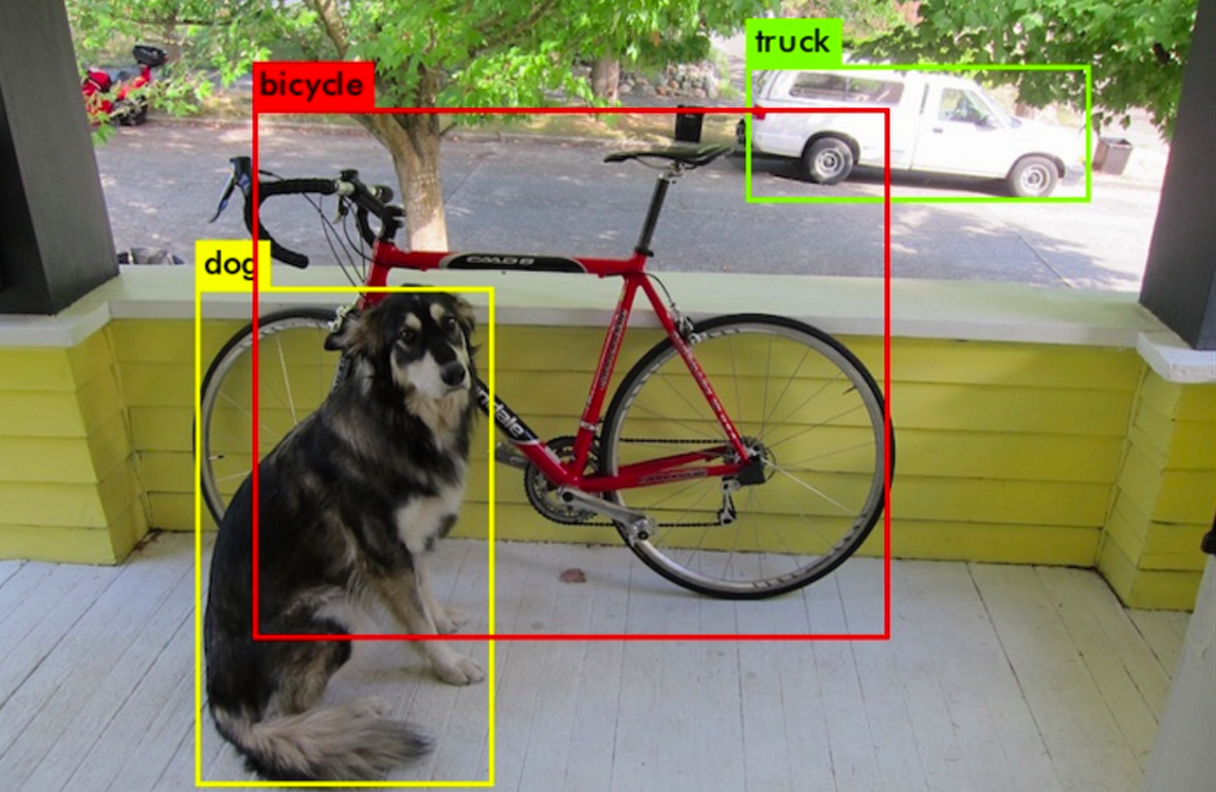
\includegraphics[scale=0.25]{images/object-detection.png}
    \caption{In the image, the detected objects are enclosed by bounding boxes \\and annotated with their corresponding class labels}
    \label{fig:object-detection}
\end{figure}

To evaluate object detection performance, the \textbf{Intersection over Union (IoU)} metric~\cite{ibm_what_2024} is commonly employed. IoU quantifies the overlap between a predicted bounding box and the corresponding ground-truth bounding box. It is defined as the ratio between the area of intersection and the area of union of the two bounding boxes:

\begin{equation}
\mathrm{IoU} = \frac{\mathrm{Area}(B_p \cap B_{gt})}{\mathrm{Area}(B_p \cup B_{gt})}
\end{equation}
where $B_p$ denotes the predicted bounding box and $B_{gt}$ the ground-truth bounding box.
IoU serves as a fundamental metric for assessing localization accuracy.

In addition to evaluation, IoU is also used during post-processing stages of object detection pipelines. Modern detection architectures often generate multiple bounding box proposals for a single object.
To eliminate redundant detections and retain only the most reliable prediction per object, a post-processing technique known as \textbf{Non-Maximum Suppression (NMS)} is applied.
NMS operates by first sorting all predicted bounding boxes according to their confidence scores in descending order. The bounding box with the highest confidence is selected as a valid detection, and all other boxes with an Intersection over Union (IoU) greater than a predefined threshold with respect to the selected box are suppressed. This process is repeated iteratively on the remaining boxes until no further candidates are available.
Formally, given a set of predicted bounding boxes $B_i$ with associated confidence scores $s_i$, NMS retains a subset of boxes such that highly overlapping detections are removed while preserving the most confident predictions. The IoU threshold plays a crucial role in determining the strictness of suppression: lower thresholds lead to more aggressive filtering, whereas higher thresholds allow more overlapping detections to remain.\\
NMS significantly improves the clarity and interpretability of detection results by ensuring that each object instance is represented by a single bounding box. 
\\

In conclusion, object detection provides a coarse yet computationally efficient form of localization, making it particularly suitable for \textbf{real-time applications} and scenarios in which precise object boundaries are not strictly required, as is the case in the present work.\\
This approach is generally designed to balance accuracy and computational efficiency, enabling their deployment in industrial environments characterized by constrained hardware resources.

